% Director-field Stokes model and the effective boundary condition behind the layer (2026-10-07 night)
\subsection{Hydrodynamics from the full active stress of the measured director field}\label{sec:dirstokes}
After the sign correction (box in Sec.~\ref{sec:hydro}) the point-defect model is replaced by the full active force of the measured director
field, with no defect idealisation and no head/tail convention (\texttt{theory/dirstokes/}). For each flow interval: $Q=S(\mathbf n\mathbf n-\mathbb I/2)$
from the director snapshots at both ends of the interval (averaged, since the flow output is an interval average), force density $\mathbf f=-\nabla\!\cdot Q$
(centred differences inside the cavity, one-sided at the wall), split into a wall band (cell centre within 4 cells of the wall) and the bulk;
Stokes flow with no slip ($\eta=1$, FEM as before) of each part; measured flow $=c_w\mathbf u_w+c_b\mathbf u_b$ fitted per run. Circles
$R=31.83$ ($k=2,6,10$, 40 intervals of 50 time units) and ellipses $\varepsilon=1.2,1.5,2.0$ (two seeds, 40 intervals of 100).
\begin{itemize}
  \item \textbf{One positive coefficient explains most of the flow.} $\mathbf v=c(\mathbf u_w+\mathbf u_b)$ gives $R^2=0.62$--0.72 in circles and
        0.48--0.65 in ellipses, circulation correlation 0.61--0.85, with $c=0.42$--0.67, against $\zeta_\mathrm{eff}/\eta\approx0.24$ from the rough
        calibration (Sec.~\ref{sec:frank}): the right sign and order of magnitude.
  \item \textbf{The bulk drives, the wall band brakes.} Alone, the bulk part gives $R^2=0.47$--0.73 with a positive coefficient; the wall band alone
        gives $R^2\le0.21$ and only with a negative coefficient, its circulation anti-correlates with the measured one ($-0.56$ to $-0.85$), and it carries
        9--17\% of the predicted circulation. The local power $\langle\mathbf f\cdot\mathbf v\rangle$ is positive in both regions, but the flow the wall
        band produces, confined by the no-slip wall, opposes the circulation.
  \item \textbf{The two vortices of elongated ellipses come from the bulk active stress.} The antisymmetric (two-vortex) part of the half-cavity
        rotations predicted by the bulk force correlates with the measured one at 0.87--0.91 ($\varepsilon=1.5$, 2.0, both seeds), and the vortex number is
        right in 72--82\% of the intervals (measured two-vortex fraction 50--68\%). The wall band opposes both the one- and the two-vortex parts.
\end{itemize}
\begin{figure}[H]\centering
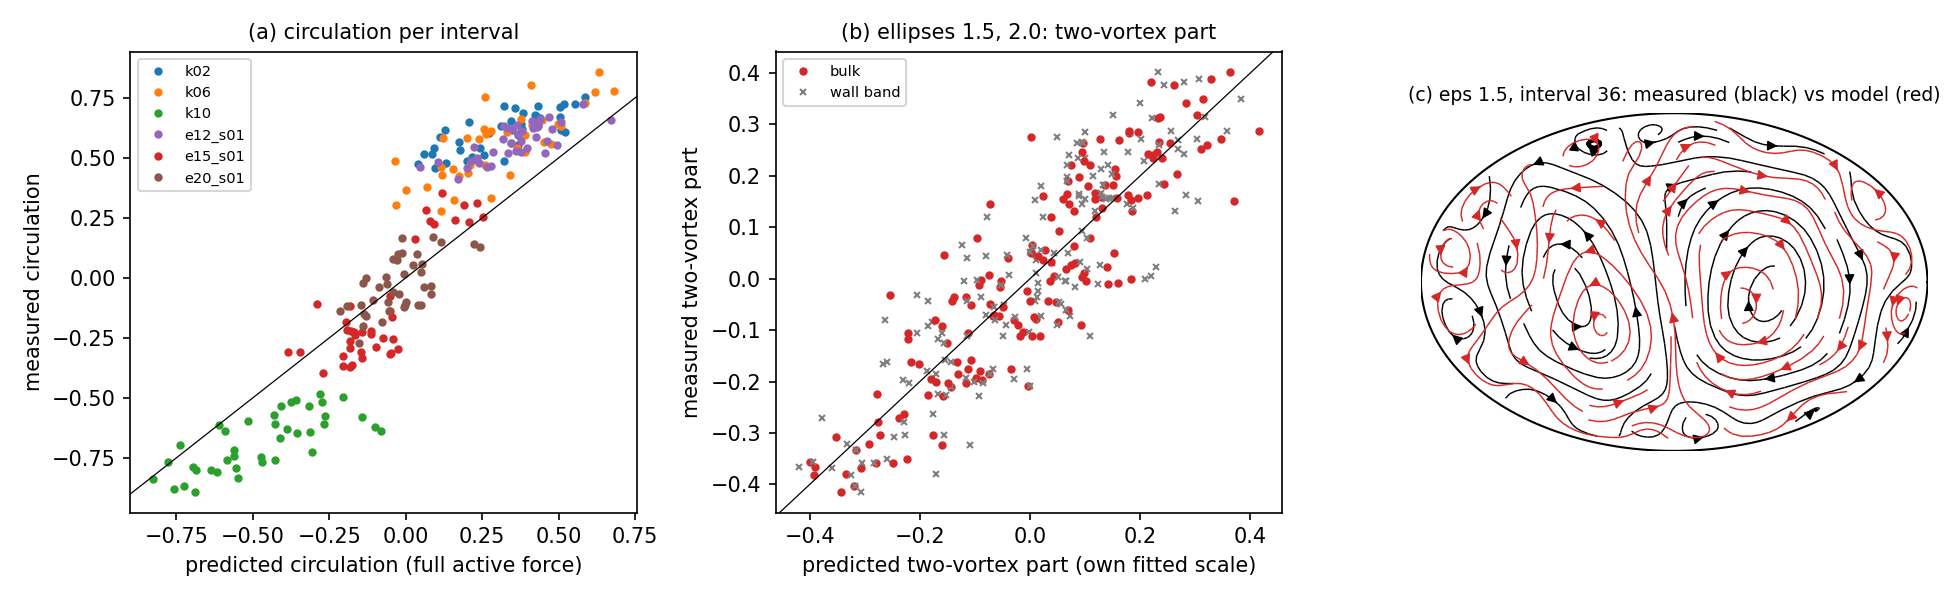
\includegraphics[width=\textwidth]{dirstokes.png}
\caption{Stokes flow of the full measured active force $-\nabla\!\cdot Q$. (a) Cavity circulation per interval, measured against predicted (one fitted
coefficient per run; circles $k=2,6,10$ and ellipses, seed 1). (b) Ellipses $\varepsilon=1.5$, 2.0 (both seeds): two-vortex (antisymmetric) part of the
half-cavity rotations, measured against the bulk-only prediction (red) and the wall-band-only prediction (grey; its fitted scale is negative: the wall band
opposes the measured flow). (c) An interval with two vortices at $\varepsilon=1.5$: measured (black) and predicted (red) streamlines.}\label{fig:dirstokes}
\end{figure}

\subsection{The wall layer as an effective planar boundary}\label{sec:effbc}
\emph{Question (B.~Loewe):} how closely spaced must the tilted wall defects be to act as an effective (planar) boundary condition, and does that give
an independent criterion for the $+1$ bulk? In the one-constant solution the layer's field inside the ring splits into a uniform part
$q_i\arg(-z_i)$ summed over the ring and a modulation that decays as $(r/r_\mathrm{ring})^N\approx e^{-2\pi\delta/\ell}$ with the depth $\delta$ behind the layer
($\ell=2\pi r_\mathrm{ring}/N$, $N=2k-2$). With the anchoring of the code ($\theta=k\phi$ on the wall, \texttt{lc.c}) and the measured registry (tails at the
wall, sites at $\phi_j=2\pi j/N$), the bulk $+1$ sees $\theta=\phi+c$ with (\texttt{theory/effbc/effective\_bc.py}, exact for $k=3,6,10$):
\begin{itemize}
  \item $c=90^\circ$ for an untilted layer: the layer converts the $k$-fold patterned anchoring into an \textbf{effectively planar} (tangential)
        condition of winding 1, the parallel-anchoring problem of Norton \emph{et al.};
  \item $c=90^\circ+\tau/2$ for a layer tilted by $\tau$ (registry shift $\tau/(2k-2)$): a spiral, $121.5^\circ$ at the measured $\tau=63^\circ$;
  \item the modulation falls below 0.1 rad at $\delta=0.25\,\ell$ for every $k$: the bulk sees a smooth effective boundary from $\approx0.34\,\ell$ from the
        wall (ring depth included), i.e.\ at a fraction $2.1/N$ of the radius.
\end{itemize}
\textbf{Self-consistency.} For an extensile $+1$ with $\theta=\phi+c$ the active force has an azimuthal component $\propto\sin(2c-180^\circ)$:
zero for the planar condition, positive (counter-clockwise) for $c=121.5^\circ$. The tilt sign follows the circulation (tilt $+63^\circ$ with counter-clockwise
flow), so a tilted layer turns the effective boundary into a spiral whose active stress drives the same circulation that tilts the layer: a feedback that
runs through the elastic field behind the layer, not through point forces at the wall (which oppose the flow, Sec.~\ref{sec:dirstokes}).

\textbf{Spacing criterion against the data} (main circle sweep, 151 $(\rho,k)$ points, $k\ge2$, $\rho\le0.15$, seed means;
\texttt{spacing\_criterion.py}, Fig.~\ref{fig:spacing}). In this sweep $R=k/\pi\rho$, so the spacing $\ell\approx1/\rho$ at any $k$ and lines of constant $k$ are
diagonals in the $(R,\ell)$ plane.
\begin{itemize}
  \item \textbf{The existence of a bulk charge is set by size, not spacing:} $R/\ell_a\ge0.76$ classifies 99\% of the points (AUC 0.997), the spacing alone
        only 80\% (AUC 0.59); adding a spacing bound ($\ell\le2.25\,\ell_a$) gains one point.
  \item The excess bulk charge at large radii (the less-charged layer, $q>1.25$) is also set by size, $R/\ell_a\gtrsim2.2$, at any spacing.
  \item Spacing matters for the \emph{pinning} of the layer on the crowded side: lattices with $\ell\lesssim0.4\,\ell_a$ at small $R$ are not pinned.
  \item Within the sweep ($\ell/\ell_a=0.3$--3) the spacing therefore does not provide an independent criterion for the $+1$ bulk. The effective-boundary
        picture does predict that $k=2$ ($N=2$, smoothing depth $\approx R$) never sees a clean planar boundary: the single $k=2$ point in the range
        $R/\ell_a=0.8$--2.2 has a density-criterion bulk charge of 0.44 against 1.0 for every $k\ge3$ (suggestive; one point).
\end{itemize}
\begin{figure}[H]\centering
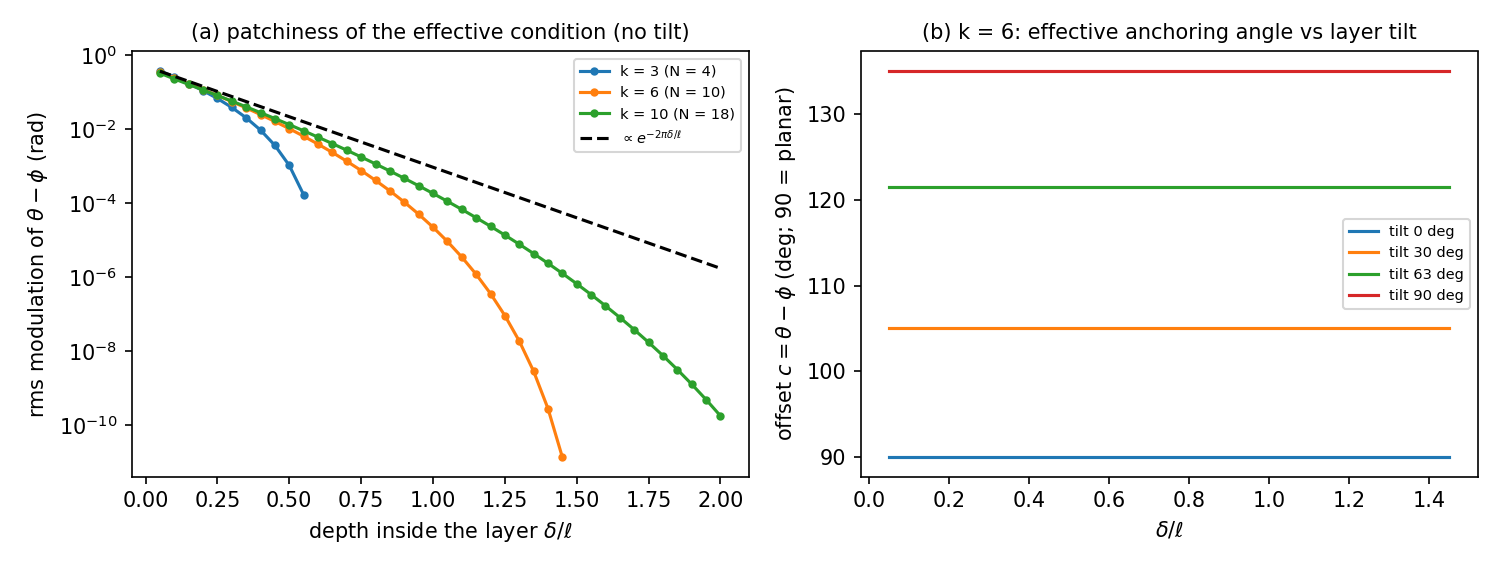
\includegraphics[width=0.9\textwidth]{effective_bc.png}
\caption{Effective boundary condition behind the wall layer (one-constant theory, $R=31.83$, central $+1$). (a) rms modulation of $\theta-\phi$ against
the depth behind the layer in units of the spacing, untilted layer, $k=3,6,10$; dashed: $e^{-2\pi\delta/\ell}$. (b) $k=6$: effective anchoring angle
$c=\theta-\phi$ (90$^\circ$ = planar) for layer tilts 0--90$^\circ$: $c=90^\circ+\tau/2$.}\label{fig:effbc}
\end{figure}
\begin{figure}[H]\centering
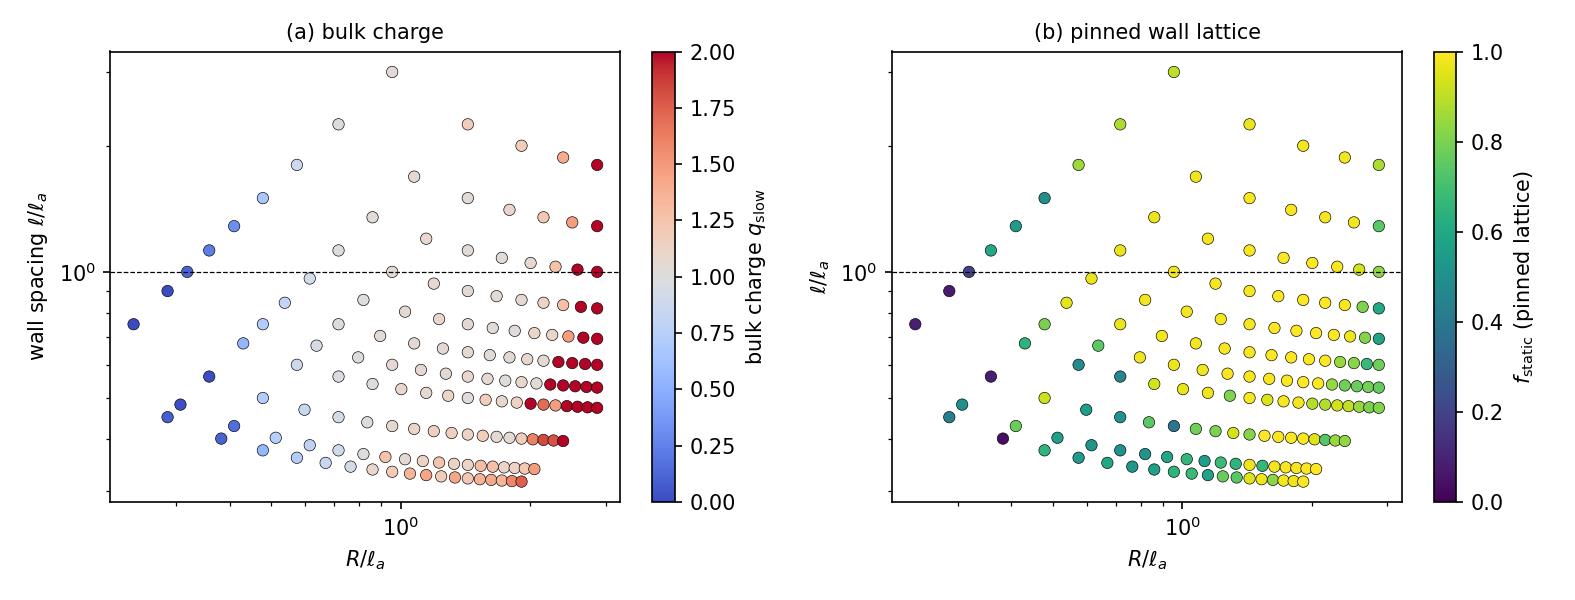
\includegraphics[width=0.9\textwidth]{spacing_criterion.png}
\caption{Main circle sweep in the plane of size $R/\ell_a$ and wall spacing $\ell/\ell_a$ (log axes; diagonals are constant $k$). (a) Bulk charge
(mobility criterion). (b) Pinned fraction of the wall lattice.}\label{fig:spacing}
\end{figure}

\subsection{A particle (defect Langevin) model: what it misses}\label{sec:defectmodel}
\emph{Idea (B.~Loewe):} each defect with its own overdamped Langevin equation, interacting elastically and as Stokeslets
(\texttt{theory/defectmodel/}). Minimal version: the $2k$ $+\half$ only (no creation or annihilation, so the observed state of $2k-2$ wall $+\half$ and a
bulk $+1$ is reachable); elastic force from the exact disk energy with images ($K=K_3$, $\mu=0.02$, thermal noise); orientation slaved to the positions
through the one-constant field (head $=-e^{2i\theta_\mathrm{rest}}$, the measured tilt lock); self-propulsion $v_0$ along the head; each $+\half$ a
point force $f$ along its head in the no-slip disk (exact Green's function, precomputed once on the unit disk, scale-free in 2D; reciprocity error 0.04\%).
Scan at $k=6$, $R=31.83$: $v_0=0.02$--0.3, $f/\eta=0$--3.
\begin{itemize}
  \item Below $v_0\approx0.1$ all 12 stay at the wall; from $v_0\approx0.15$ most leave at once (wall count 3--8): no stable $2k-2$ + $+1$ state.
  \item The circulation stays $\le0.02$ (measured 0.4--0.7) and changes sign constantly: point forces of a ring of $+\half$ largely cancel.
  \item Missing physics: the wall binding of a $+\half$ is far stronger than the log energy (orientation-dependent, the 80--110\,$k_BT$ anisotropy barrier of
        Sec.~\ref{sec:fluct}); self-propulsion is suppressed at a no-slip wall; and the circulation is driven by the distributed bulk active stress
        (Sec.~\ref{sec:dirstokes}), which a point-force model of the defects does not carry. A useful particle model needs at least an orientation-dependent
        wall potential and the $+1$ spiral stress of Sec.~\ref{sec:effbc}.
\end{itemize}

\paragraph{Adding the spiral flow to the particle model} (B.~Loewe's suggestion; \texttt{defect\_langevin.py}, \texttt{scan\_spiral.py},
\texttt{scan\_structured.py}). At every step the mean tail tilt $\tau$ of the wall defects sets the effective boundary $c=90^\circ+\tau/2$; whenever the
wall holds $2k-2$ defects (inner winding 1) the spiral body force $(\zeta/\eta)S\sin\tau/r$ ($(\zeta/\eta)S=0.48$, calibrated) acts on
$r_c<r<R-0.34\ell$ and its exact axisymmetric no-slip flow advects all defects.
\begin{itemize}
  \item \textbf{Free model} ($k=6$, $R/\ell_a=1.43$): the spiral flow matters only when the $2k-2$ + bulk $+1$ state exists. At $v_0=0.15$ this state is
        present 27--30\% of the time and the circulation then rises to 0.29--0.38 (0.007 without the spiral), but the state is not stable (wall defects still
        leave in avalanches), so the circulation flips and the tilt has no consistent sign.
  \item \textbf{Given the structure} (the $2k-2$ wall defects held radially at the layer depth, free along the wall, with the calibrated anisotropy
        pinning; the bulk pair free but kept 6 cells from the wall, because nothing in the log energy holds a $+1$ in the bulk, the passive ground state being
        $2k$ at the wall): the loop produces a circulation and a tilt that follows it. $k=6$: no circulation up to $R/\ell_a=0.6$ ($\le0.07$, tilt
        $\le10^\circ$); from 0.8, circulation 0.40, 0.65, 1.0, 1.6 at $R/\ell_a=0.8$, 1.0, 1.43, 2.0 with tilt$\times$sign(circulation) $=+24^\circ$ to
        $+29^\circ$. Without the spiral: circulation $\le0.014$, tilt $\approx5^\circ$ with no sign rule. $k=4$: onset between 0.8 and 1.0 (circulation 0.19,
        0.51, 1.07 at 0.8, 1.0, 1.43; tilt $+19^\circ$ to $+39^\circ$). The sense of rotation reverses over time, as in the simulations.
  \item Compared with the MPCD circles: circulation of the right size (0.65--1.0 against 0.6 at $R/\ell_a=1.43$), tilt smaller (30--40$^\circ$ against
        $63^\circ$), onset later ($\approx0.7$ against 0.39--0.44), and the predicted $k$-ordering (onset at larger $R/\ell_a$ for $k=4$ than for $k=6$). What keeps
        the $+1$ in the bulk, and the wall defects at the wall, remains outside the model.
\end{itemize}

\paragraph{What sets the size of the tilt: splay $\neq$ bend beyond first order} (B.~Loewe's question; \texttt{theory/aniso2/}).
In the particle model the tilt is not locked: it wanders (10--90\% range $-59^\circ$ to $+49^\circ$), the layer slips 2.4 sites per 1500 time units and the
circulation reverses often, whereas the MPCD layer sits at $\pm63^\circ$ without creep. A stable intermediate tilt needs a minimum of the tilt potential away
from zero, i.e.\ a term with a different $\tau$-dependence than the drive ($\propto\sin\tau$).
\begin{itemize}
  \item \textbf{To first order in $K_1-K_3$ this is impossible, exactly:} a registry shift rigidly adds $\tau/2$ to the one-constant director, so
        $\int(\text{splay}^2-\text{bend}^2)$ is exactly $\propto\cos\tau$ (numerically: $-66$, $-44$, $-22\,k_BT\cos\tau$ for $k=4,6,8$, all higher harmonics zero). The
        bulk $+1$ adds another $\cos\tau$ term (it prefers the pure-bend vortex: $\approx-46\,k_BT\cos\tau$ at $k=6$).
  \item \textbf{Beyond first order:} the director was relaxed under the full anisotropic Frank energy ($K_1=42$, $K_3=23.1$; correction field vanishing at the wall,
        rigid defect cores, energy outside the cores; \texttt{relax\_frank2.py}; check $K_1=K_3$: flat to a residual $0.8\,k_BT\cos2\tau$). $k=6$, $R=31.83$:
        $E(\tau)\approx-(31\text{--}47)\cos\tau+(4.6\text{--}7.6)\cos2\tau-(1\text{--}3)\cos3\tau$ $k_BT$, the sign of the $\cos2\tau$ term the same for core radius 1.5
        or 2.5, grid 0.5 or 0.35, point or paired bulk $+1$, cores fixed or free. (A first version with soft core weights failed its check and was discarded.)
  \item \textbf{This sign gives a stable tilt.} With a drive torque $D\sin\tau$, the net torque is $\sin\tau\,[D-|A_1|+4A_2\cos\tau]$: the untilted layer becomes
        unstable at $D_c=|A_1|-4A_2$ and the tilt grows continuously (supercritical) as $\cos\tau^*=(|A_1|-D)/(4A_2)$; above $D=|A_1|+4A_2$ the layer slides.
  \item \textbf{Particle model with the second harmonic} (\texttt{scan\_a2.py}; structured, $k=6$): the tilt locks where the drive is moderate. With $A_2=20\,k_BT$:
        $|\tau|=64^\circ$ (59--68$^\circ$, 99\% of the time in 45--80$^\circ$, no slip, no reversals) at $R/\ell_a=1.0$ and half the calibrated spiral drive;
        $67^\circ$ at $R/\ell_a=0.6$ with the full drive. $A_2=10$: $\approx49^\circ$; $A_2=5$ (the computed value): $\approx35^\circ$. With the full calibrated drive
        at $R/\ell_a\ge0.8$ the layer slides for every $A_2$.
  \item \textbf{Reading.} Splay $\neq$ bend supplies the missing ingredient qualitatively: a $\cos2\tau$ term of the right sign that turns the onset into a
        supercritical bifurcation with a locked finite tilt. Quantitatively the elastic estimate ($A_2\approx5$) gives $\approx35^\circ$; the measured $63^\circ$
        needs $A_2\approx15$--20, or a further contribution of the same harmonic (core energy of a tilted $+\half$ at a homeotropic wall, flow alignment). The
        calibrated drive is too strong for locking in the larger cavities, consistent with the missing brake of the wall band (Sec.~\ref{sec:dirstokes}),
        which the particle model does not contain.
\end{itemize}

\paragraph{Flow alignment} (B.~Loewe's question; \texttt{theory/flowalign/}). The MPCD nematic rotates each particle's orientation by Jeffery's rule,
$\dot{\mathbf u}=\mathbf u\cdot W+\lambda(\mathbf u\cdot D-\mathbf u\,\mathbf u\mathbf u\!:\!D)$ (Larson), with $\lambda=$ \texttt{tumble} $=2$, the rotation rate scaled
by \texttt{shearSusc} $=0.5$ (\texttt{lc.c}, \texttt{jefferysTorque}): flow aligning, Leslie angle $\tfrac12\arccos(1/\lambda)=30^\circ$ from the flow. None of the models
above contains it. Measured (active circles $R=31.83$, $k=2,6,10$, 64 snapshots each; director minus the one-constant field of the measured defects, signed by
the circulation):
\begin{itemize}
  \item \textbf{A non-elastic, flow-signed residual.} $-1^\circ$ at the wall, growing inwards to $-25^\circ$ at 6--10 cells ($k=6,10$; $-10^\circ$ at $k=2$); within 6 cells
        of the wall its size grows with the local shear ($\approx5^\circ$ at the weakest, 10--12$^\circ$ at the strongest) and its sign follows the sign of the shear.
  \item \textbf{Small at the wall layer, large in the bulk.} At the depth of the wall defects (1--2 cells) the residual is only 4--5$^\circ$: flow alignment barely rotates
        the wall defects, so it does not add tilt directly.
  \item \textbf{It erases the elastic spiral in the bulk.} The elastic field of the measured defects predicts a bulk spiral at $122$--$123^\circ$ from radial ($90^\circ+\tau/2$);
        the measured director is at $110^\circ$ 2--6 cells from the wall and $74^\circ$ ($k=6$), $87^\circ$ ($k=10$) in the bulk ($0.3$--$0.7R$): close to tangential.
  \item \textbf{Where the drive actually is.} The measured azimuthal active force (from $-\nabla\!\cdot Q$, signed by the circulation) has a net positive torque, located in a
        ring just inside the layer, $r/R\approx0.6$--0.9 (3--12 cells from the wall; the smoothing zone of the effective boundary is $\approx0.34\ell\approx6$ cells), negative
        in the wall band ($r/R>0.9$, the brake) and slightly negative in the inner bulk ($0.2$--$0.5R$). The effective-boundary drive exists but is confined to an
        annulus behind the layer; deeper in, flow alignment turns the director back towards tangential.
  \item \textbf{Consequences for the particle model.} The $1/r$ spiral force over $r_c<r<R-0.34\ell$ overestimates the drive (consistent with locking needing about half the
        calibrated drive) and puts it in the wrong place; the next version should use the measured annular drive, and flow alignment of the bulk texture.
\end{itemize}

\paragraph{Annular-drive particle model: a closure test that fails, and why} (\texttt{defectmodel/scan\_annular.py}).
The drive was replaced by the measured one: the effective azimuthal body force $f_\mathrm{eff}(r)=-(v''+v'/r-v/r^2)$ reconstructed from the measured mean swirl of the
$k=6$, $R=31.83$ circle (it agrees with $c\,\langle-\nabla\!\cdot Q\rangle_\phi$ in the driving ring, $r/R=0.7$--0.85, and has a weaker wall-band brake), scaled by
$\sin\tau/\sin63^\circ$ so that the model reproduces the measured flow exactly at the measured tilt; no defect Stokeslets (the profile contains all active forces);
structured layer, $B=90\,k_BT$, $A_2=0$--20.
\begin{itemize}
  \item \textbf{The tilt does not lock at $63^\circ$.} With the calibrated drive the median $|\tau|$ is 26--29$^\circ$ with a broad distribution, the layer slips by up to
        $130^\circ$ per 1000 time units and the circulation reverses 20--40 times; more drive gives less tilt (faster sliding), half the drive 37--55$^\circ$, still broad.
  \item \textbf{Why: in MPCD the wall defects are not carried by the flow.} The fluid at the layer depth moves at 0.13--0.16 cells per time unit (signed with the circulation),
        the wall $+\half$ at $0.0005\pm0.0010$ ($k=6$) and $0.0004\pm0.0005$ ($k=10$): an effective advection coefficient of 0.002--0.004, zero within error. The layer sits
        at a static, shifted registry ($\pm\tau/(2k-2)$ for $\pm63^\circ$); the anchored texture between the defects and the wall holds it. In the model the wall
        defects move with the fluid (0.2--0.4 cells per time unit), and the registry pinning can hold at most $\mu F\approx0.03$, so the layer slides.
  \item \textbf{Consequence.} The tilt is not produced by the flow continuously pushing the layer; it is a static state reached at the reversals. The next version
        needs the kinematics of a wall defect (a texture anchored to the wall, advection coefficient $\ll1$, to be measured from the registry jumps at reversals), after
        which the torque balance of Sec.~\ref{sec:effstab} applies with $D$ replaced by the static drag on the layer.
\end{itemize}

\subsection{Stability of the untilted layer through the effective boundary}\label{sec:effstab}
Loop (\texttt{theory/stability/effbc\_stability.py}): a registry shift $\alpha$ of the layer tilts it by $\tau=(2k-2)\alpha$ (measured lock); the bulk then sees
a spiral boundary $c=90^\circ+\tau/2$, whose extensile stress exerts $f_\phi=(\zeta/\eta)S\sin\tau/r$ in the smooth region $r_c<r<R-0.34\ell$; the axisymmetric
no-slip Stokes flow advects the layer, $\dot\alpha=v(r_s)/r_s$; the anisotropy pinning restores it at the rate $\mu E''/(Nr_s^2)$ (Sec.~\ref{sec:fluct}). Linear
growth rate $\lambda=(2k-2)(\zeta/\eta)S\,h-\mu E''/(Nr_s^2)$, $h$ the dimensionless advection of the layer per unit spiral drive (0.016--0.025).
\begin{itemize}
  \item With the calibrated $\zeta/\eta=0.42$--0.67 (director-field fit), $S=0.876$, $\mu=0.02$ and $E''$ from the anisotropy calculation, the untilted layer is
        unstable above $R/\ell_a\approx0.47$--0.50 ($k=6$), 0.4 ($k=8$), 0.6--0.75 ($k=4$), for a bulk-core radius $r_c=0.25\,\ell_a$: the size at which the measured
        circulation and tilt appear (0.39--0.44). Small cavities stay untilted because the pinning rate grows as $1/r_s^2$.
  \item The onset depends on the assumed core radius ($k=6$: 0.30--0.63 for $r_c=0$--0.4\,$\ell_a$); the robust prediction is the ordering, onset at smaller
        $R/\ell_a$ for larger $k$. The main sweep measures the onset only for $k=2$--4 (0.46, 0.39, 0.40; larger $k$ start above it), which neither confirms
        nor rejects the ordering; the defect-only tilt coherence is too noisy at small $N$. Decisive test: circulation of the small high-$k$ cavities
        ($\rho=0.16$--0.5, flows to be reduced on the server).
\end{itemize}

\subsection{Site arrangement, curvature and the second vortex}\label{sec:sitecurv}
\paragraph{Moving the pinned sites inside the circle} (B.~Loewe's idea; branch \texttt{anchmod}, \texttt{runs/anchmod\_test}). A sine-modulated winding
$\theta_\mathrm{wall}=k\phi+A\sin(m\phi)$ (eMode 2; \texttt{anchAmp}, \texttt{anchMode}, \texttt{anchPhase}; validated: $A=0$ reproduces production bit for bit, $A=1$
gives a wall director within $9^\circ$ rms of $6\phi+\sin\phi$) makes the homeotropic points, $(k-1)\phi+A\sin(m\phi)\equiv0$ (mod $\pi$), unevenly spaced while the
wall curvature and the topology stay those of the circle.
\begin{itemize}
  \item \textbf{Active (final, 9 runs, $\approx1000$ time units of production):} the wall sites sit within 0.21--0.27 cells (rms) of the predicted modulated
        homeotropic points shifted by the tilt, 2.2--4.5 cells from the best evenly spaced lattice; gaps 17--25 cells ($A=1$, $m=1$) and 14.6--30 cells ($A=1$, $m=2$);
        runs with the same sense of rotation agree within 0.06--0.13 cells whatever the initial director; opposite senses differ by 7.6 cells ($=2\tau/(2k-2)$). Tilt
        63--64$^\circ$. The anchoring pattern sets the active sites (\texttt{anchmod\_results.txt}).
  \item \textbf{Passive (3 runs): not pinned by the modulation} (my prediction was wrong). The three initial directors give site sets 3.3--8.5 cells apart. Reason: a
        modulation $A\sin(m\phi)$ couples to the ring through $\sum_je^{im\phi_j}$, which vanishes for $2k=12$ evenly spaced defects unless $m$ is a multiple of 12; $m=1,2$
        only distort the gaps (13.9--20.3 cells against 16.7 uniform) and leave the rotation free. The active ring is pinned by splay $\neq$ bend at the homeotropic points
        wherever they are; the passive one is not.
  \item \textbf{Geometry or topology: the layer does not depend on where its sites are.} Sweep with flow output (\texttt{runs/anchmod\_sweep}: $m=1$, $A=1,2,3$;
        $m=2$, $A=1,1.5,2$; 2 seeds each; random start), scored with \texttt{theory/anchmod/layer\_observables.py} against 10 uniform-circle runs: bulk charge
        0.75--0.87 (baseline 0.76--0.83), 10 wall defects in 85--97\% of the frames (88--93\%), tilt 61--63$^\circ$ with coherence 0.96--0.97 (63--64$^\circ$, 0.97), no
        reversals, no escapes (one run 0.05 per 1000 time units), circulation 0.59--0.75 (0.62--0.75), never two vortices. Moving the pinned sites by up to several cells
        leaves every property of the layer unchanged: the layer is robust to the site arrangement. The ellipse instability therefore does not come from the uneven
        arrangement of the sites but from the curvature or the elongated flow (these circles never form a second vortex, so the circle sweep alone does not separate those two;
        the ellipse analysis below does).
\end{itemize}

\paragraph{Is the second vortex what breaks the layer in ellipses?} (B.~Loewe's hypothesis; \texttt{theory/vortexlayer/}.) A single vortex asks for a uniform tilt, i.e.\
a rigid registry shift; two counter-rotating vortices ask for opposite tilts on the two halves, i.e.\ opposite shifts that compress the lattice where the vortices meet the
wall on one side and stretch it on the other, a natural source of vacancies and escapes. Test on the active ellipses (W3, two seeds): per flow interval, one or two
vortices; escapes = wall $+\half$ followed for 20 time units (nearest-neighbour chains) that end deeper than 6 cells (a first version counting single-frame escapes had too
few events and was discarded).
\begin{table}[H]\centering\small
\caption{Escape probability of a wall $+\half$ within 20 time units, and mean number of vacancies, in one- and two-vortex intervals (1500--2700 escapes per state at
$\varepsilon\ge1.5$). Meeting region: $|x|<A/4$, where the two vortices meet the wall; tips: $|x|>A/2$.}\label{tab:vortexlayer}
\begin{tabular}{lccccc}\toprule
& state & escape prob. & meeting region & tips & vacancies\\\midrule
$\varepsilon=1.2$ & one vortex (always) & 0.005 & 0.004 & 0.006 & 0.22\\
$\varepsilon=1.5$ & one vortex & 0.072 & 0.038 & 0.104 & 2.31\\
 & two vortices & 0.066 & 0.049 & 0.080 & 2.31\\
$\varepsilon=2.0$ & one vortex & 0.070 & 0.066 & 0.081 & 2.70\\
 & two vortices & 0.077 & 0.076 & 0.093 & 2.73\\\bottomrule
\end{tabular}
\end{table}
\begin{itemize}
  \item \textbf{No instantaneous link.} At $\varepsilon\ge1.5$ the layer is $\approx14\times$ leakier than at $\varepsilon=1.2$ in both vortex states; vacancies are the same; the
        two-vortex indicator and the escape rate are uncorrelated at lags from $-200$ to $+200$ time units ($|r|\le0.11$).
  \item \textbf{Escapes concentrate at the tips}, not where two vortices meet the wall.
  \item \textbf{Reading.} Elongation, most likely the tip curvature, weakens the layer at all times and also allows the second vortex: two consequences of the geometry rather
        than cause and effect. Caveat: the vortex state switches every few hundred time units, and slow healing could hide a time-integrated effect. The circle sweep above
        (uneven sites, no tips) separates the two: an intact circle layer would point to curvature, a leaking one to the site arrangement.
\end{itemize}

\subsection{Response of the wall layer to an imposed vortex and its reversal}\label{sec:swirl}
(B.~Loewe's suggestion; \texttt{theory/reversals/swirl\_response.py}.) An optional azimuthal body acceleration was added to the solver (branch \texttt{anchmod},
\texttt{bin/mpcd\_swirl.out}; inputs \texttt{swirlAcc}, \texttt{swirlRadius}, \texttt{swirlX/Y}, \texttt{swirlFlipTime}, \texttt{swirlPeriod}; production steps only;
switched off it reproduces production bit for bit). Runs: $k=6$, $R=31.83$, acceleration within $0.6R$ (away from the layer), reversed at production time 1500.
\begin{table}[H]\centering\small
\caption{Imposed swirl and its reversal. Circulation and tilt before $\to$ after; times of their zero crossings after the reversal; registry shift of the layer
(measured, and predicted by the tilt lock $\Delta\tau R_l/N$).}\label{tab:swirl}
\begin{adjustbox}{max width=\textwidth}
\begin{tabular}{lcccccc}\toprule
run & circulation & fluid at layer & tilt (deg) & $t_0$ circ., tilt & registry shift (lock) & transit\\\midrule
active, $A=0.005$ & $+0.79\to+0.40$ & $+0.16\to+0.06$ & $+64\to+64$ & not reversed & $-0.1$ ($0$) & --\\
active, $A=0.01$ & $+0.97\to-0.93$ & $+0.16\to-0.17$ & $+65\to-65$ & 375, 678 & $-7.2$ ($-6.8$) & 344, from $+448$\\
active, $A=0.02$ & $+1.13\to-1.15$ & $+0.16\to-0.16$ & $+66\to-66$ & 295, 384 & $-7.3$ ($-7.0$) & 42, from $+380$\\
passive, $A=0.003$ & $+0.18\to-0.18$ & $+0.02\to-0.02$ & $+57\to-57$ & 115, 236 & $+4.4$ (slides) & --\\
passive, $A=0.01$ & $+0.49\to-0.49$ & $+0.06\to-0.06$ & $+63\to-59$ & 105, 210 & $+40$ (slides) & --\\
passive, $A=0.02$ & $+0.74\to-0.74$ & $+0.09\to-0.09$ & $+68\to-66$ & 85, 164 & $+44$ (slides) & --\\\bottomrule
\end{tabular}
\end{adjustbox}
\end{table}
\begin{itemize}
  \item \textbf{The active vortex resists a weak reversal} ($A=0.005$: circulation reduced but not reversed, tilt unchanged): the self-sustained state is bistable.
  \item \textbf{The active layer is a stick--slip system.} It stays at its registry until the flow at its depth has reversed, then jumps by the amount the lock predicts
        ($-7.2$, $-7.3$ cells against $-6.8$, $-7.0$) within 42--344 time units, and locks at the mirror registry. The tilt lags the circulation by 90 time units at the
        stronger drive, as at the spontaneous reversals of circles (Sec.~\ref{sec:hydro}). The near-zero advection in the steady state (Sec.~\ref{sec:effstab}) is
        pinning, not insensitivity to the flow.
  \item \textbf{A passive layer under imposed flow tilts too, to $\pm57$--$68^\circ$}, nearly independent of the flow strength (fluid at the layer 0.02--0.09), and
        slides with the flow (40--44 cells; the passive ring is not pinned). In the active cavities the tilt is an active effect (the only flow there is the active
        flow), but its \emph{angle} appears to be set by the response of the wall layer to the presence of flow.
  \item \textbf{The angle is controlled by the flow-alignment parameter} (\texttt{runs/swirl\_tumble}, passive, imposed swirl, \texttt{tumble} $\lambda$ changed): final tilt
        $\approx28$--$36^\circ$ at $\lambda=0.5$ (tumbling), 57--65$^\circ$ at $\lambda=1.2$ (43$^\circ$ after the reversal at the stronger drive), 57--68$^\circ$ at $\lambda=2$,
        75--83$^\circ$ at $\lambda=4$. The tilt grows monotonically with $\lambda$, so it is set by the flow alignment of the nematic at the wall; the simple guess
        $2\theta_L=\arccos(1/\lambda)$ (34$^\circ$, 60$^\circ$, 76$^\circ$) fails at $\lambda=1.2$, and the tumbling case still tilts, so the agreement at $\lambda=2$, 4 is not
        evidence for it. The active runs all use $\lambda=2$.
\end{itemize}
\begin{figure}[H]\centering
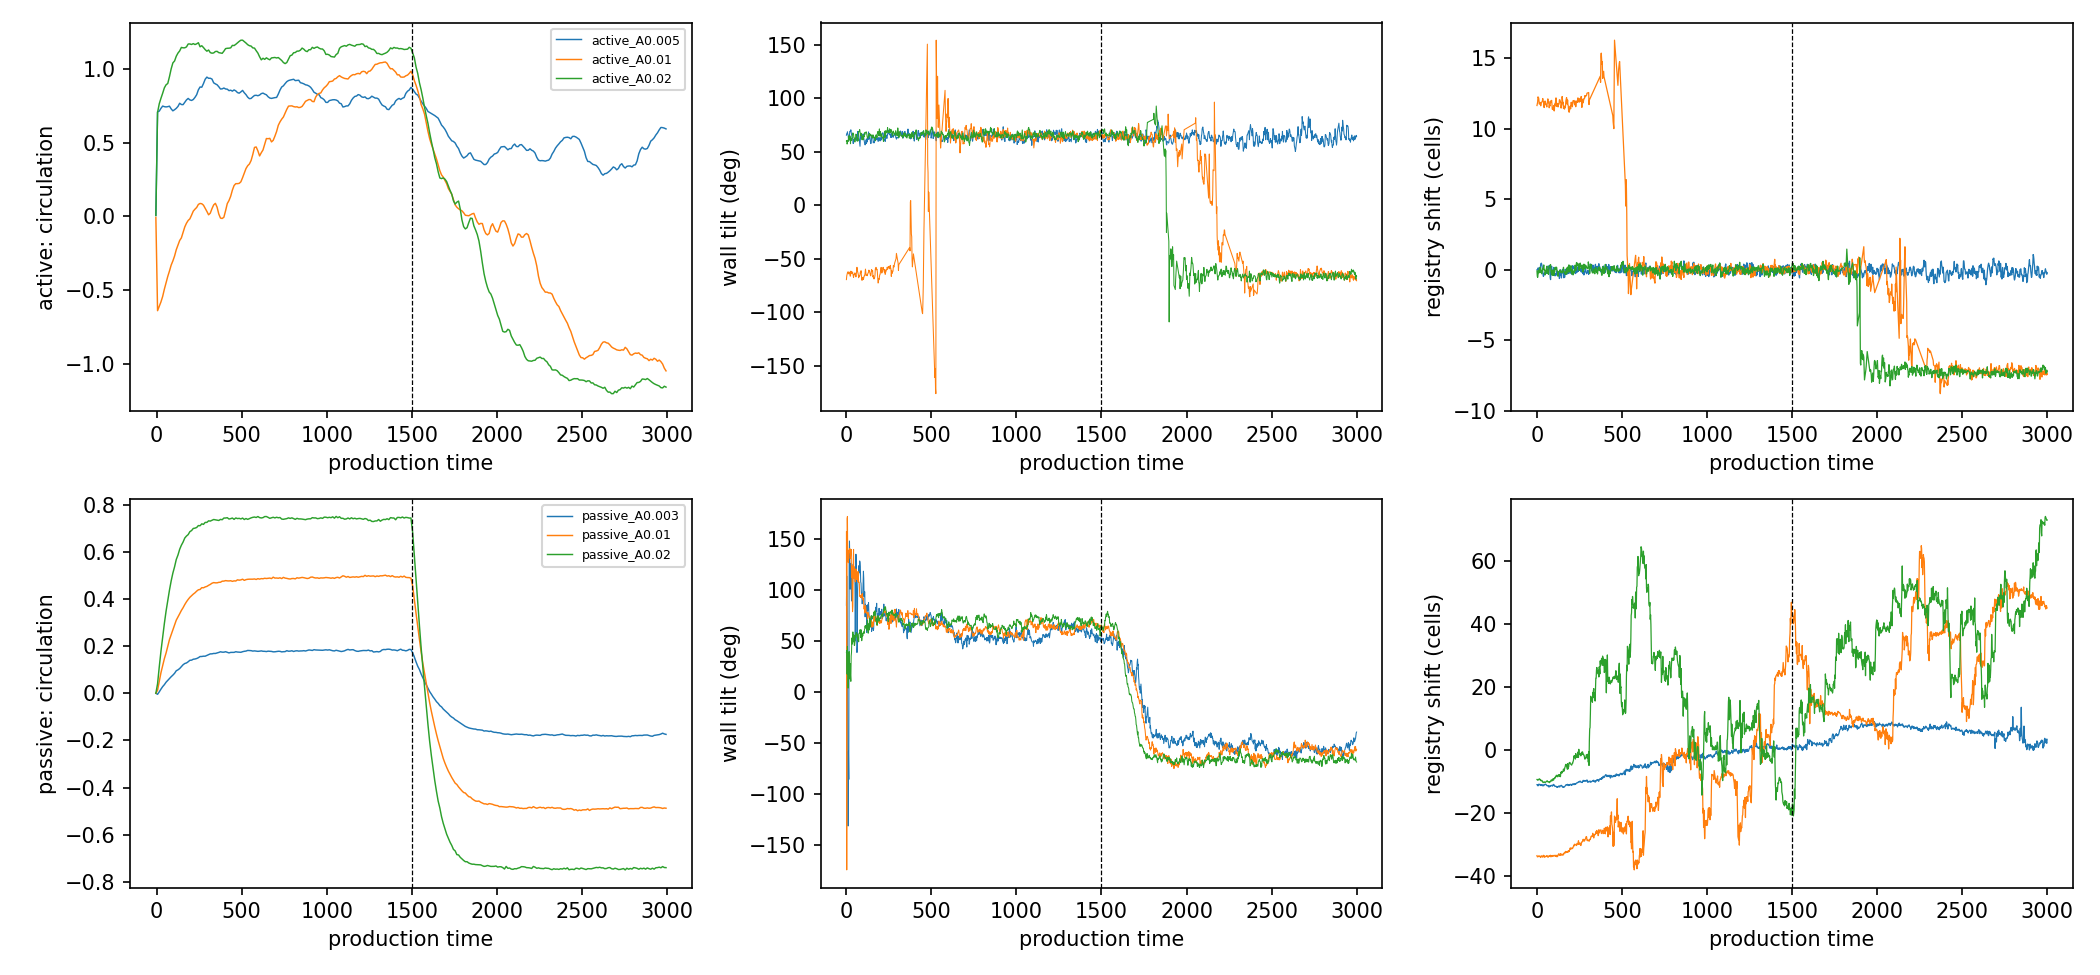
\includegraphics[width=\textwidth]{swirl_response.png}
\caption{Imposed swirl reversed at production time 1500 (dashed). Top: active; bottom: passive. Circulation, wall tilt and registry shift of the layer.}\label{fig:swirl}
\end{figure}

\subsection{Half-integer windings}\label{sec:halfk}
A nematic allows half-integer $k$: the wall director $k\phi$ returns to itself up to a sign after one turn, and the code's anchoring is insensitive to that sign
(the particle orientation is projected on the imposed director). The pattern then has an odd number, $2k-2$, of homeotropic points and no inversion symmetry.
Runs: $k=0.5$, 1.5, 2.5, 3.5, 5.5, $R=31.83$, active (2 seeds) and passive (1), production binary (\texttt{runs/halfk}; \texttt{theory/halfk/analyse\_halfk.py}).
\begin{itemize}
  \item \textbf{$k\ge2.5$ behaves exactly like integer $k$.} Active: $2k-2=3$, 5, 9 wall $+\half$ in 85--93\% of the frames; registry on the odd set of homeotropic
        points (lock-corrected $D=0.00\pm0.09$, concentration 0.99--1.00); tilt 63--65$^\circ$, coherence 1.00; bulk charge as for integer $k$; one steady vortex
        (circulation 0.66--0.74, no reversals). The integer references ($k=2$--6, same $R$): 2--10 wall defects, tilt 59--65$^\circ$, circulation 0.62--0.74. An odd
        number of sites and the missing inversion symmetry change nothing.
  \item \textbf{$k=1.5$ (one wall site predicted): no layer.} The wall stays empty (0.04 wall $+\half$ on average); the charge $3/2$ sits in the bulk (about three $+\half$,
        bulk charge $\approx1.25$); the flow is weak and erratic (circulation 0.08--0.12, 6--7 reversals). One defect cannot make a smooth effective boundary (its smoothing
        depth, $\approx2R$, exceeds the radius; Sec.~\ref{sec:effbc}). $k=2$ (two sites, smoothing depth $\approx R$) still forms its layer.
  \item \textbf{$k=0.5$:} no layer; a single $+\half$ circulates in the bulk at $\approx0.6R$ and drives a strong, steady vortex (0.42--0.49, at most one reversal).
  \item \textbf{Passive:} consistent with the depth law. At $k=0.5$ the single $+\half$ sits near the centre (the law gives $r^*=0$); for $k=1.5$--3.5 the predicted ring is
        deep (6.7--2.6 cells) and straddles the 4-cell wall band; at $k=5.5$ all 11 sit at the wall with the frustrated tilt pattern of a $2k$ ring.
\end{itemize}

\subsection{Flow-induced ejection: why the active wall holds $2k-2$}\label{sec:ejection}
\emph{Mechanism (B.~Loewe):} the vortex means flow; flow tilts the wall defects; the tilted $2k$ ring becomes too expensive and two defects leave.
\paragraph{Energetics} (\texttt{theory/ejection/}; rigid cores of radius $a$, director relaxed outside them; one-constant $K=32.5$ and anisotropic $K_1=42$,
$K_3=23.1$; $k=4,6,8$, $R=31.83$). A: the $2k$ ring. B: a $2k-2$ ring (bulk charge 1) plus two $+\half$ at $\pm0.45R$; both contain the same $2k$ defects, so core
energies cancel. Flow alignment is modelled by forcing every wall core to the same tilt $\tau$. Validation: unrelaxed, one-constant, $\tau=0$ with natural cores,
$E_B-E_A=+183.7\,k_BT$ numerically against $+184.0$ from the image formula.
\begin{itemize}
  \item \textbf{Without flow the $2k$ ring is stable:} ejecting two defects costs $+155$ to $+200\,k_BT$ (all $k$, both elasticities, $a=1.5$, 2.5).
  \item \textbf{A common tilt frustrates the $2k$ ring.} Its natural tilts wind around it ($150^\circ,90^\circ,30^\circ,\dots$ at $k=6$; Sec.~\ref{sec:status}); forcing them
        equal costs $+375$ to $+475\,k_BT$ at $k=6$ ($+200$ to $+510$ for $k=4$--8), nearly independent of the value of $\tau$. The $2k-2$ ring takes a common tilt by a registry shift, almost for free
        ($<40\,k_BT$).
  \item \textbf{Under a common tilt the ejected structure is cheaper} by 20--330\,$k_BT$, for every $k$, both elasticities and both core sizes (the magnitude depends on
        the core size, the sign does not).
\end{itemize}
\paragraph{Direct test: passive cavities under imposed flow eject two defects.} In the passive imposed-swirl runs (Sec.~\ref{sec:swirl}; no activity) the wall goes
from 12 to 10 $+\half$ and the bulk acquires charge $+1$: $\lambda=2$, $A=0.003$: $12\to11\to10$ (bulk $0\to0.5\to0.8$); $A=0.01$, 0.02: $12\to10$ (bulk $\to0.9$--1.0);
$\lambda=4$, both $A$: $12\to10$ (bulk 1.0). $\lambda=1.2$: only partly, at the stronger drive ($12\to11$, bulk 0.5); $\lambda=0.5$ (tumbling, no aligned angle): never.
The tilts measured in those runs ($\pm57$--$83^\circ$) are those of the 10-defect ring left after the ejection.
\paragraph{Reading.} The structure of the active cavities, $2k-2$ wall $+\half$ and a bulk $+1$, follows from flow plus flow alignment: flow imposes a common tilt on the
wall defects, a $2k$ ring cannot take a common tilt (its tilts must wind), so two defects leave into the bulk, leaving the largest ring that can tilt uniformly. Activity
enters by providing the flow. This links the onset of the bulk charge to the onset of a coherent flow, and predicts that a nematic with a smaller flow-alignment parameter
holds more defects at the wall under the same flow.
\begin{figure}[H]\centering
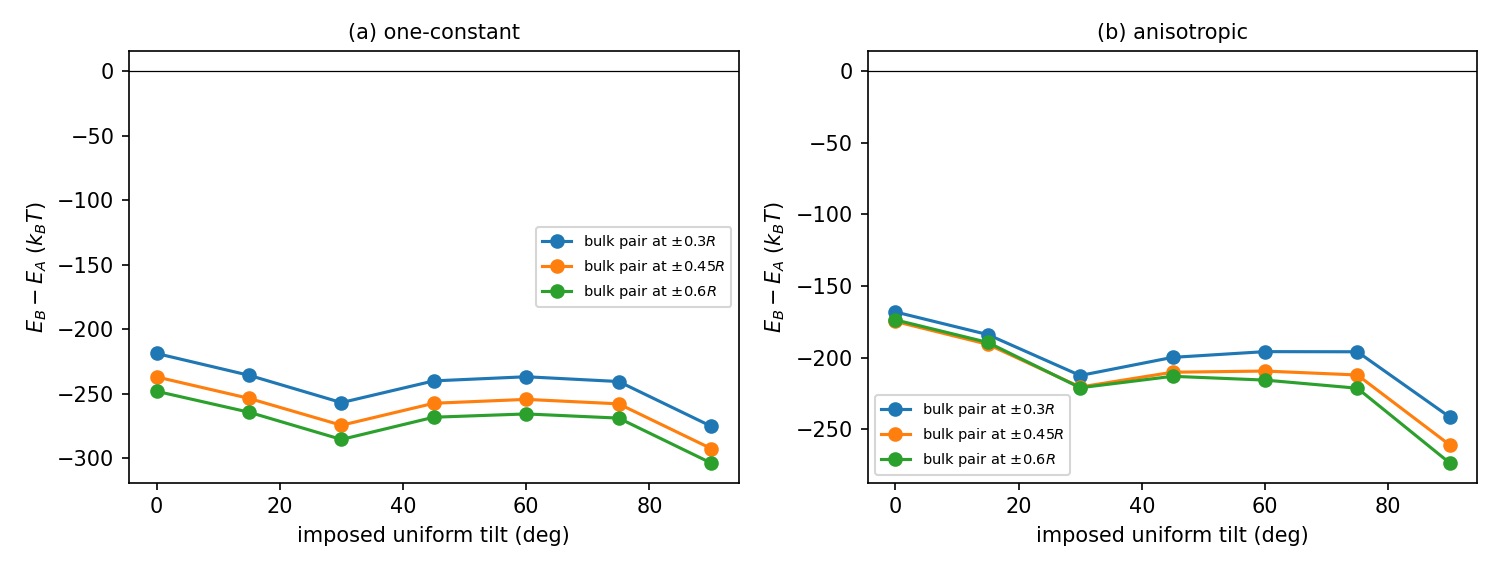
\includegraphics[width=0.9\textwidth]{tilted_structures.png}
\caption{Energy of the ejected structure (B: $2k-2$ ring plus a bulk pair) minus the $2k$ ring (A), both with every wall core forced to the same tilt, $k=6$,
$R=31.83$, for three positions of the bulk pair; (a) one-constant, (b) anisotropic. Negative: ejection favoured. (Baseline without forcing, natural tilts:
$E_B-E_A\approx+180\,k_BT$.)}\label{fig:ejection}
\end{figure}

\subsection{Ejection threshold and the negative layer}\label{sec:ejection2}
\begin{itemize}
  \item \textbf{Threshold} (\texttt{runs/swirl\_threshold}; passive circle $k=6$, $R=31.83$, constant swirl, 2 seeds; \texttt{theory/overnight/}): no ejection up to $A=0.003$ in
        3000 time units (wall 12, tilt coherence 0.2--0.5, circulation/$v_\mathrm{rms}$ up to 0.77); at $A=0.01$ both seeds eject two (wall 10, bulk $+0.75$, $+0.93$) and the tilt
        coherence jumps to 0.90--0.96. The ejection needs a flow strong enough to impose a common tilt; a reversal helps (the reversed $A=0.003$ run of
        Sec.~\ref{sec:swirl} ejected).
  \item \textbf{Negative layer} ($k=-6$, $R=28.21$, passive, imposed swirl; \texttt{theory/ejection/ejection\_neg.py}). Energetics: the commensurate 14-ring
        ($2|k-1|$) has uniform natural tilts ($\pm60^\circ$: one arm into the bulk), the 12-ring's wind; under a common tilt the 14-ring plus a bulk $+1$ is cheaper by
        196--392\,$k_BT$ minus the core cost of a created $\pm\half$ pair. Simulation: the wall stays at 12 $-\half$ for $\lambda=0.5$, 2; only $\lambda=4$ reaches 13. Gaining
        $-\half$ needs pair creation in the bulk, rare without activity: kinetically blocked, not refuted. A fair test needs activity or a seeded pair.
\end{itemize}

\subsection{Shapes: the sweep through the circle framework}\label{sec:shapesweep}
Server sweep (675 runs: Cassini ovals $b/a=1.1$--3.0, ellipses $\varepsilon=1.2$--2.5, circles; $R_\mathrm{eq}=1.0$, 1.5, 2.0\,$\ell_a$; five densities; 3 seeds;
\texttt{theory/shapes/}).
\begin{itemize}
  \item \textbf{One transition, set by the aspect ratio alone.} Tilt coherence, circulation and the single-vortex state collapse together at aspect 1.25--1.37, for ellipses and
        ovals at every size (Fig.~\ref{fig:phaseshapes}); the long semi-axis at the transition ranges from 1.2 to 2.3\,$\ell_a$, so no length sets it. Below it the cavity behaves
        like a circle (no vacancies, bulk $\approx+1$, coherence 0.92--0.94, one vortex); above it vacancies 1.5--2.9, bulk charge 1.4--2.0, coherence 0.39--0.63, circulation
        0.04--0.30, two vortices 32--84\% of the time, escapes 15--20$\times$.
  \item \textbf{Above it the layer loses more with size}: about 1, 3 and 4.5 vacancies at $R_\mathrm{eq}=1.0$, 1.5, 2.0\,$\ell_a$ (bulk charge 1.1, 1.8, 2.5).
  \item \textbf{The local lock survives everywhere} (0.91--0.97): what fails is the occupancy of the layer and the coherence of the flow.
  \item \textbf{Escapes} (pooled, by local wall curvature): rise at $\kappa R_\mathrm{eq}\gtrsim1.25$, but non-circular cavities leak 5--10$\times$ more than circles even at
        circle-like curvature: part global, part local.
  \item \textbf{Tips.} Measured effective potential of wall $+\half$ ($-\ln P(\text{depth})$, in units of the active noise; same noise at tips and flanks checked): wells
        25--35\% shallower at the tips at $\varepsilon\ge1.5$, consistent with the 2--2.5$\times$ faster escapes there; not set by the vortex number; not explained by static
        elasticity ($\approx8\%$) nor by a tilt misfit (the local lock holds at every site). With lock-produced tilts, one vortex weakens the tips by 1--2\,$k_BT$ and two vortices
        weaken the flanks (their meeting points) by 3--4\,$k_BT$, as observed at the flanks; the tip weakness in two-vortex intervals remains unexplained.
\end{itemize}
\paragraph{Is the deficit caused by the loss of coherent flow? Not settled.}
\begin{itemize}
  \item \emph{Passive ellipses with an imposed single vortex} (\texttt{runs/swirl\_ellipse}): at $\varepsilon=1.5$ the wall goes 12$\to$10, the bulk gains $+1$, the tilt becomes
        coherent: with a coherent flow an ellipse behaves like a circle; curvature alone does not prevent the $2k-2$ layer.
  \item \emph{Active ellipses with an imposed vortex}: the layer is not repaired (wall 7--8, bulk 1.5--1.7, two vortices 36--56\% of the time) even when the imposed swirl brings
        the circulation to 0.57--0.66\,$v_\mathrm{rms}$.
  \item \emph{Per interval} (450 elongated runs, 22\,500 intervals): the wall count does not follow the instantaneous flow ($|r|\le0.05$ with the circulation, $\le0.15$ with the
        tilt coherence, any lag; same vacancies with one or two vortices). In circle-like cavities it does ($r=+0.25$).
  \item \textbf{Not decisive.} The imposed vortex never made the active ellipses circle-like coherent (tilt coherence 0.62--0.64 against 0.97 in circles; two vortices still
        36--40\% of the time), so activity disrupting the coherent flow (B.~Loewe) remains a viable explanation of the deficit; the interval correlations argue against it only
        weakly, since elongated cavities may never reach circle-like coherence. Tests running: stronger imposed vortices (swirl 0.06, 0.1) in active ellipses, and vacancies binned
        by tilt coherence. Alternatives: escape/refill kinetics at the curved tips; the bulk defect population.
\end{itemize}
\begin{figure}[H]\centering
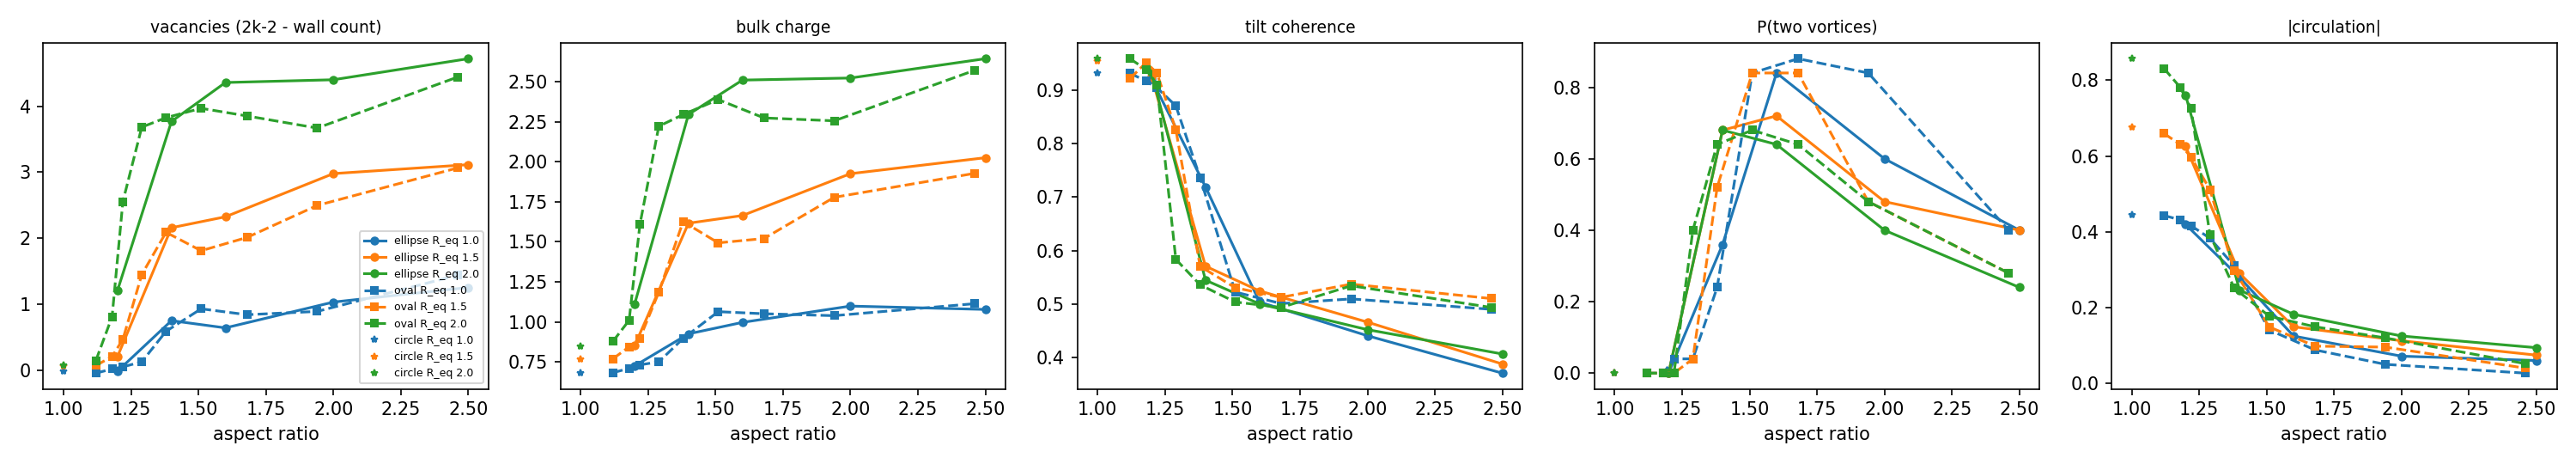
\includegraphics[width=\textwidth]{phase_shapes.png}
\caption{Shape sweep: vacancies, bulk charge, tilt coherence, probability of two vortices and circulation against the aspect ratio, for ellipses (solid) and ovals (dashed) at
$R_\mathrm{eq}=1.0$, 1.5, 2.0\,$\ell_a$ (colours); stars: circles. Medians over $k$, densities and seeds.}\label{fig:phaseshapes}
\end{figure}


\subsection{The tilt angle: flat no-slip wall in shear}\label{sec:tiltangle}
(\texttt{theory/shear\_tilt/}: \texttt{flatwall.py}, \texttt{flatwall\_scan.py}, \texttt{mpcd\_profile.py}, \texttt{solvability.py}.) Question (B.~Loewe): does the no-slip shear set the
tilt, and can its value ($\approx62^\circ$) be computed? Local limit: a flat wall at $y=0$, simple shear $v_x=sy$ (no slip), periodic along the wall with one site spacing $a_s$.
\paragraph{Equations.} Director angle $\theta(x,y)$ from the wall direction; anchoring $\theta(x,0)=\pi/2+qx$, $q=\pi/a_s$ (homeotropic at $x=0$, a rotation by $\pi$ per
period, screened by one $+\half$ at depth $d$). One-constant Ericksen--Leslie in the director limit,
\begin{equation}
\gamma_1(\partial_t+\mathbf v\cdot\nabla)\theta = K\nabla^2\theta+\gamma_1\frac{s}{2}\left(\lambda\cos2\theta-1\right),\label{eq:el}
\end{equation}
($-s/2$: rotation with the vorticity; $\lambda\frac s2\cos2\theta$: strain alignment; aligned angle $\cos2\theta_L=1/\lambda$, stable for $\lambda>1$).
\paragraph{Step 1: the layer is a zero mode.} At $s=0$, $\theta$ is harmonic. If $\theta_0(x,y)$ is a solution with the defect at $x=0$, then
$\theta_D(x,y)=\theta_0(x-D,y)+qD$ satisfies the same anchoring ($\theta_w(x-D)+qD=\theta_w(x)$) and has the same energy $\frac K2\int|\nabla\theta|^2$: a one-parameter
family. Translating the defect by $D$ rotates the far field by $\theta_\infty=qD$, and near the core ($\theta\simeq\frac12\arg(z-z_D)+c_D$, $c_D=c_0+qD$) rotates the comet axis
by $2qD$. Hence $\tau=2\theta_\infty=2\pi D/a_s$: the tilt--position lock (Sec.~\ref{sec:status}) is this zero mode.
\paragraph{Step 2: leading order.} Beyond the screening length $a_s/2\pi$ the texture is uniform along $x$ (corrections $\propto e^{-2\pi y/a_s}$) and \eqref{eq:el} reduces
to $K\theta''=-\gamma_1\frac s2(\lambda\cos2\theta-1)$. Its only bounded stable state is $\theta=\theta_L$. If the near-wall region transmits no torque, the outer
region is uniformly aligned, the layer sits on the zero mode with $\theta_\infty=\theta_L$, and
\begin{equation}
\tau_0=2\theta_L=\arccos(1/\lambda),
\end{equation}
independent of $s$, $K$ and $\gamma_1$ (the angle is set by the ratio of strain to vorticity in simple shear, which the no-slip wall fixes).
\paragraph{Step 3: boundary-layer correction.} Linearising the outer problem about $\theta_L$, $\theta=\theta_L+\delta$:
$K\delta''=\gamma_1 s\sqrt{\lambda^2-1}\,\delta$, so $\delta=\delta_0e^{-y/\ell_E}$ with the alignment length $\ell_E=\sqrt{K/(\gamma_1 s\sqrt{\lambda^2-1})}$. A torque $\Gamma$ per
unit length passed from the near-wall region gives $K\delta'=-\Gamma$, i.e.\ $\delta_0=\Gamma\ell_E/K$. \emph{Ansatz:} in the band $0<y<d$ between the wall and the defects the
director follows the winding anchoring ($\langle\cos2\theta\rangle\approx0$ over a period), so its alignment torque averages out and only the vorticity acts,
$\Gamma=\gamma_1 sd/2$, transmitted in full to the layer (the band moves with the zero mode). Then
\begin{equation}
\tau=\arccos\frac1\lambda+d\sqrt{\frac{\gamma_1 s}{K}}\,(\lambda^2-1)^{-1/4}.\label{eq:tilt}
\end{equation}
The correction grows as $\sqrt s$ (weak dependence on the flow strength) and diverges towards tumbling ($\lambda\to1$).
\paragraph{Tests.} (i) Flat-wall Q-tensor simulation ($L=a=\Gamma=1$, so $K/\gamma_1=1$): far field $2\theta_\infty=2\theta_L$ within $1^\circ$;
registry$\times360^\circ$ = tilt (zero mode); $s\to0$: $\tau\to\arccos(1/\lambda)$ (61.8 vs $60^\circ$ at $\lambda=2$, 49.5/48.2 at 1.5, 76.9/75.5 at 4). Eq.~\eqref{eq:tilt} with the
measured depth, no free parameter, over 35 runs ($\lambda=1.1$--4, $s=10^{-3}$--$10^{-1}$, $a_s=10$--40): measured/predicted correction 0.97 (median), correlation 0.98.
(ii) Removing the shear from the band next to the wall (rigid rotation there, the wall slips) raises the tilt by $\approx30^\circ$ (disk model), as the vorticity term of the ansatz implies.
\paragraph{Caveat: crowded layers tilt less (2026-10-15, open).} The law has no wall-density dependence, and the $\lambda$ scan tests it only in sparse layers
($\rho=k/\pi R\approx0.045$--0.09). In the main circle sweep ($\lambda=2$, $0.8\le R/\la\le2.2$) the tilt of the coherent layer ($C>0.9$, 10 seeds) falls steadily with $\rho$: 64.6$^\circ$
($\rho\approx0.04$), 63.0$^\circ$ (0.065), 54.7$^\circ$ (0.10), 44.2$^\circ$ (0.14; spacings down to $\lesssim17$ cells), while the flat-wall model shows no spacing
dependence for $a_s=10$--40. To check with the 10-seed sweep: tilt vs coherence, $|\langle v_\theta\rangle|$ and wall count (neighbour interactions vs weaker shear vs
measurement noise). The clean trend suggests a derivable correction. \textbf{First check (10 seeds, \texttt{theory/tiltcrowd/tilt\_crowding.py, plot\_tilt\_k.py}):} the drop is real, not a measurement effect. In frames where the layer is fully coherent
($C>0.9$) the tilt still falls from $64.6^\circ$ ($\rho\approx0.04$) to $44^\circ$ ($\rho\approx0.14$), and defects at the mean spacing drop as much as the layer.
The tilt collapses on the wall-defect spacing $2\pi R/(2k-2)$ (residual 1.7$^\circ$ against a raw spread of 7$^\circ$; $k$ or $R$ alone leave 5--6$^\circ$):
$\approx64^\circ$ for spacings $\gtrsim20$ cells, $60^\circ$ at $\approx15$, $\approx42^\circ$ at 7 cells; small cavities sit slightly below at equal spacing. TODO: does the smaller tilt help denser windings hold their layers (released fraction 0.61 at
$q=0.02$, 0.10 at $q=0.07$)? Tension: escapers untilt first, so a smaller tilt alone should favour escape.

\paragraph{Status of the derivation.} Steps 1--2 and the boundary-layer form of step 3 are derived. The transmitted torque $\gamma_1sd/2$ is an ansatz confirmed numerically
but not derived: projecting the full torque density onto the zero mode over the static texture (\texttt{solvability.py}) does not reproduce it (wrong sign once advection is
included, wrong $\lambda$ dependence); the projection is dominated by the region next to the core, where the fixed-$S$ director description fails. Open.
\paragraph{Mapping to MPCD.} MPCD rotates each particle by Jeffery's equation with Bretherton parameter $\lambda$ (\texttt{larsonRotRate}); \texttt{shearSusc} multiplies vorticity
and strain alike, so it changes the rate, not the angle. For $\dot\psi=-\frac s2(1-\lambda\cos2\psi)$, the moment $\langle e^{2i\psi}\rangle=S_2e^{2i\theta}$ obeys
$\dot\theta=-\frac s2\left[1-\lambda\frac{1+S_4}{2S_2}\cos2\theta\right]$, so $\lambda_\mathrm{eff}=\lambda(1+S_4)/(2S_2)$; with a Maier--Saupe distribution at the measured
$S_2=0.83$--0.88, $\lambda_\mathrm{eff}=1.80$--1.83 ($\lambda=2$), 3.61--3.66 ($\lambda=4$), 1.08 ($\lambda=1.2$). Leading order: 56--57$^\circ$, $74^\circ$, $23^\circ$.
Measured in the passive swirl runs: the tilt equals twice the director angle at the defects' depth (65.5 and 61.6 against 63.7 and 61.0$^\circ$, $\lambda=2$), with the director in the layer
at 26--33$^\circ$ against $\theta_L=28^\circ$. Matching the measured 61--64$^\circ$ with Eq.~\eqref{eq:tilt} ($d=1.75$, $s=0.047$) needs $\gamma_1/K=0.07$--0.18; then $\lambda=4$ gives
77--79$^\circ$ (measured 83) and $\lambda=1.2$ gives 32--37$^\circ$ (measured 57, weakly coherent, near tumbling). An independent MPCD measurement of $\gamma_1$ would make this a prediction.
\paragraph{Active continuum model (2026-10-09).} Q-tensor with Stokes flow, backflow and an extensile active stress $-\zeta Q$ (\texttt{shear\_tilt/active\_bf.py},
\texttt{scan\_active2.py}; one constant, no imposed flow, started from the passive 12-ring, $k=6$, $R=31.83$): $\zeta=0.1$: a vortex (circulation 0.92), no ejection (tilt coherence
0.47); $\zeta=0.3$, 1.0 at $\lambda=2$: vortex, ejection 12$\to$10 with bulk $+1$, coherent tilt 61.7, 62.1$^\circ$ (MPCD active $\approx62^\circ$), independent of $\zeta$; $\lambda=4$:
76.5$^\circ$; $\lambda=1.2$: 37.1$^\circ$. Passive with backflow and an azimuthal body force: ejection, 65.5--65.8$^\circ$ ($\lambda=2$), 77.6$^\circ$ ($\lambda=4$). The full chain
self-organises in a continuum active nematic. (A first attempt with $\zeta\le0.03$ developed no flow.) Free $\pm\half$ mobility in the bulk from pair annihilation
(\texttt{runs/rotvisc/quench\_L96}, \texttt{theory/mobility/}): $r^2$ linear in time to annihilation, $\mu\approx0.0054$, $4\times$ below the wall-defect value 0.02.

\paragraph{Correction (2026-10-09, evening): the MPCD tilt does not follow $\lambda_\mathrm{eff}$.} Particle-level moments (\texttt{runs/tiltdiag}, \texttt{trajOut}) confirm the
Maier--Saupe $S_4$ (within 0.01 in bulk and layer; slightly higher in the cores, $\lambda_\mathrm{eff}=1.98$--2.01 there). But varying the order with the mean-field potential gives a tilt
nearly independent of it: 62.2$^\circ$ ($U=5$, bulk order 0.56), 61.5--62.4$^\circ$ ($U=10$, 0.87; also at density 10), 64.8$^\circ$ ($U=20$, 0.94), against $\lambda_\mathrm{eff}$
predictions of 61.5/56.7/58.2$^\circ$ (bulk order) and 68.5/58.7/57.2$^\circ$ (order near the cores). The data follow the bare $\arccos(1/\lambda)=60^\circ$ plus 2--5$^\circ$; the
order-near-the-cores contribution proposed above is withdrawn, and the remaining degrees are attributed to splay $\neq$ bend ($+2$--3$^\circ$ in the disk model) and the boundary layer.
Why the particle-averaged alignment does not appear in MPCD is open (\texttt{theory/tiltdiag/}). Density 40 per cell: 62.6$^\circ$ (density has no effect). Rotational viscosity, final (4 seeds, modes $m=2$--4): $\gamma_1\approx60$ (splay $62\pm2$, bend $56\pm2$), consistent with the free-defect mobility 0.0054; the boundary-layer ansatz would then add $\approx16^\circ$ in MPCD against the measured 2--5$^\circ$.

\begin{figure}[H]\centering
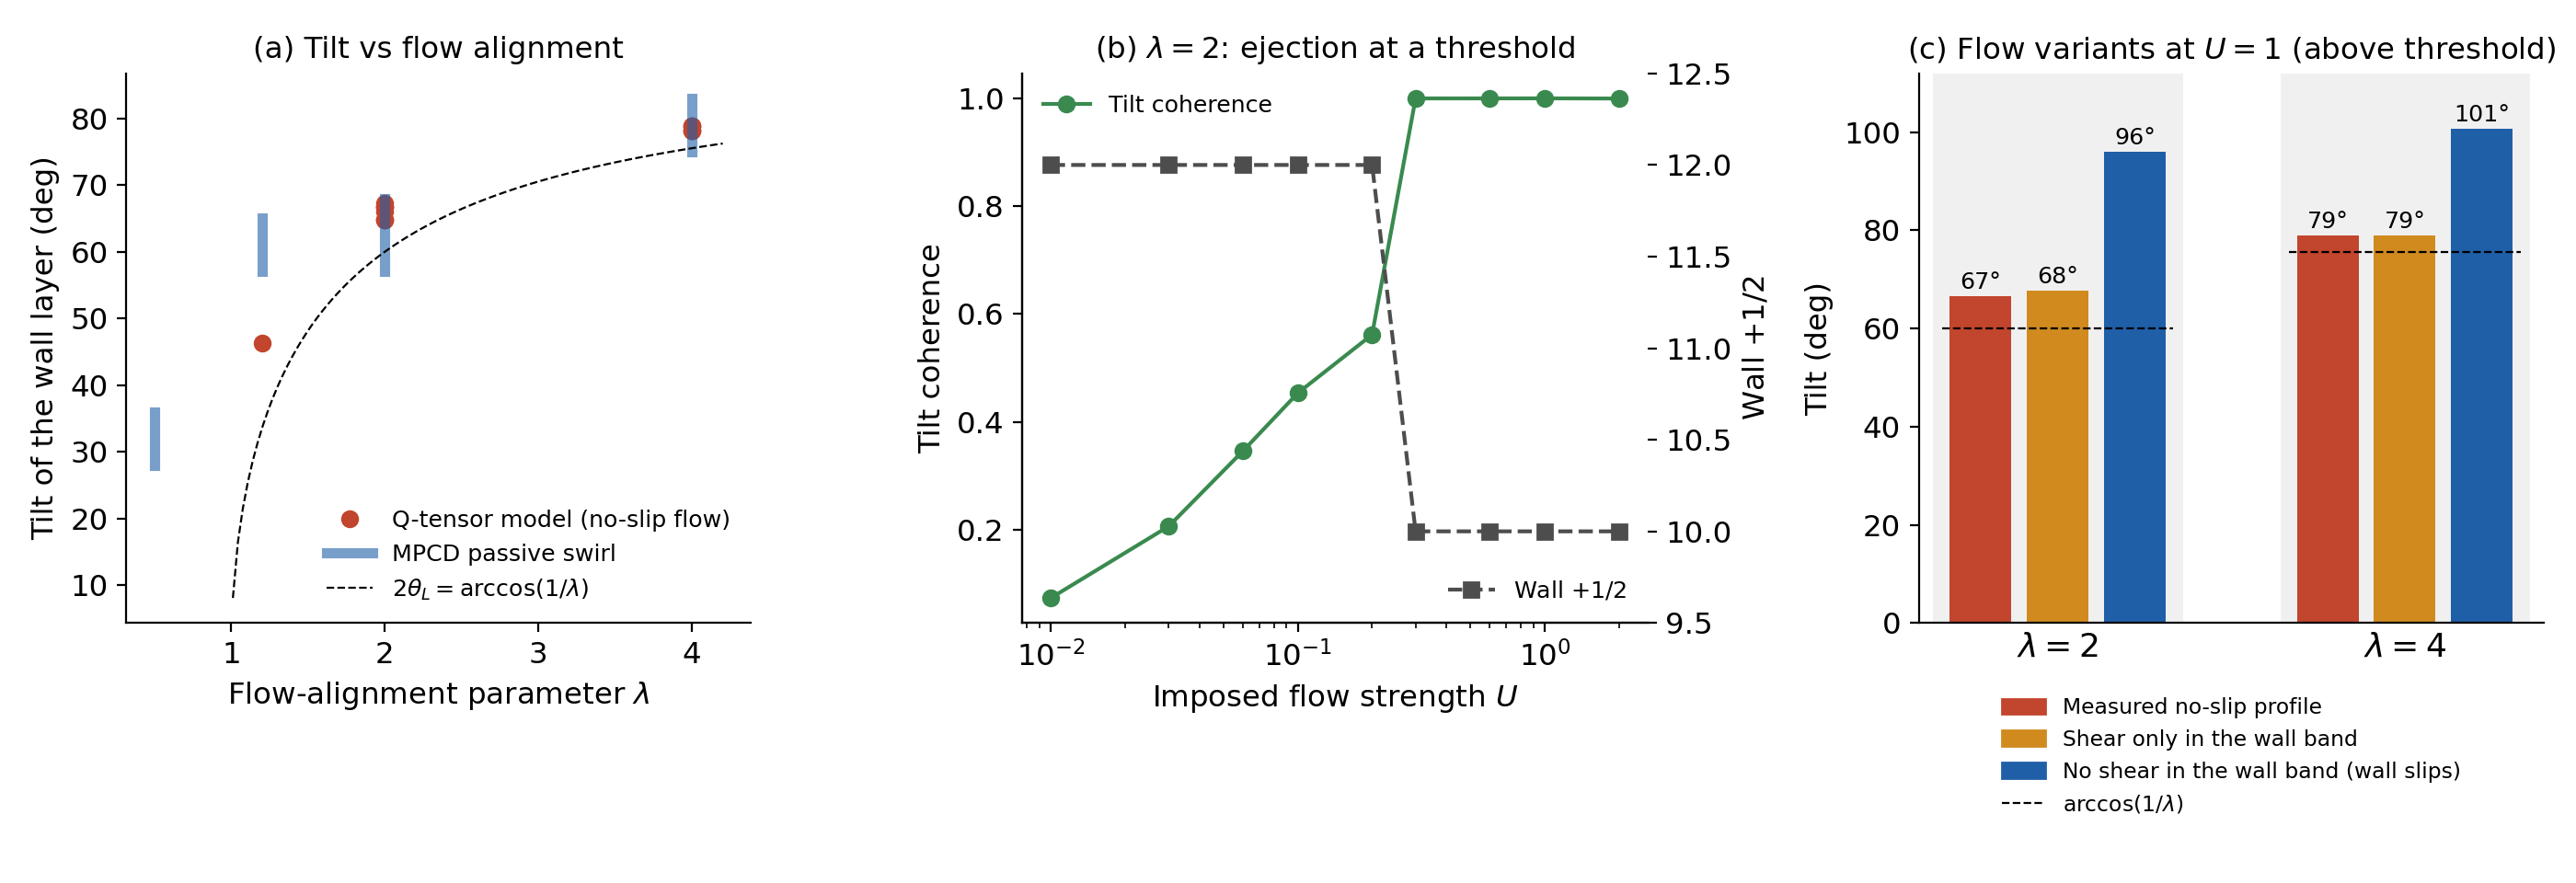
\includegraphics[width=\textwidth]{shear_tilt.png}
\caption{Disk Q-tensor model with the measured no-slip flow (one-way). (a) Tilt after ejection vs $\lambda$: model, MPCD passive swirl, $2\theta_L$. (b) $\lambda=2$: tilt coherence
and wall count vs flow strength (ejection threshold). (c) Tilt with the measured profile, shear only in the wall band, and no shear in the wall band (slip).}\label{fig:sheartilt}
\end{figure}

\subsection{Active continuum model in ellipses; bulk Leslie angle in MPCD (2026-10-10)}\label{sec:contell}
(\texttt{theory/shear\_tilt/ellipse\_active.py}, \texttt{ellipse\_runs/}; \texttt{runs/leslie/}.) The active Q-tensor model with backflow (Sec.~\ref{sec:tiltangle}) in ellipses of the
reference circle's area, arclength-uniform anchoring, $k=6$, $\lambda=2$, noise 0.005, 12\,000 time units: $\varepsilon\le1.2$ circle state at $\zeta=0.3$ and 1 (10 wall, bulk $+1$, coherence 1,
tilt 61--62$^\circ$); $\varepsilon=1.4$ circle state at $\zeta=0.3$, broken at $\zeta=1$; $\varepsilon\ge1.6$ broken (two vortices, coherence 0.48--0.54, circulation 0.18--0.31, wall 9$\to$6,
bulk $+1.5\to+3$). Transition $\varepsilon\approx1.4$--1.6 (MPCD 1.25--1.37), lower at stronger activity (Fig.~\ref{fig:contell}).
Bulk Leslie angle in MPCD (Poiseuille channel, no anchoring): $\lambda=1.2$: 17.4$^\circ$ ($U=5$, $S=0.56$), 14.2$^\circ$ ($U=20$, $S=0.95$), not aligned in half the channel at $U=10$;
$\lambda=1.5$, $U=10$: 22.3$^\circ$; $\lambda=2$, $U=10$: 29.9$^\circ$ (bare 16.8/24.1/30.0$^\circ$; particle-averaged 18.9/14.4/21.5/28.4$^\circ$). Near tumbling the alignment depends on $S$ roughly
as the particle-averaged law; at $\lambda=2$: 32.8/29.9/31.1$^\circ$ ($U=5$/10/20) vs particle-averaged 30.8/28.4/29.2$^\circ$ (offset $+1.8^\circ$). Cavity tilt = twice the measured bulk Leslie angle within $\pm3^\circ$. \emph{Self-propulsion test (continuum, $\zeta=1$):} activity off within 4 cells of the wall: vacancies 0/0/1/2/2.6/4 ($\varepsilon=1$--2.5), as without it; negative winding $k=-6$: 14 wall $-\half$ in circle-like cavities ($=2|k|+2$), 15--16 above the transition, bulk charge $+1.5$--2 in all variants: in the continuum the extra bulk charge comes from bulk activity in elongated cavities, not from self-propelled wall defects and not from the vortex number: with an imposed single vortex, activity only in the wall band or at the cores removes no defects, activity only in the bulk removes two at $\varepsilon=1.6$, 2 (two-vortex fraction 0--0.08). The MPCD wall-band switch-off is not clean (it destroys the circle's single vortex: wall 10$\to$5.5, bulk $+0.8\to+2.5$). The MPCD mirror ($-\half$ hold) stays unexplained.
\begin{figure}[H]\centering
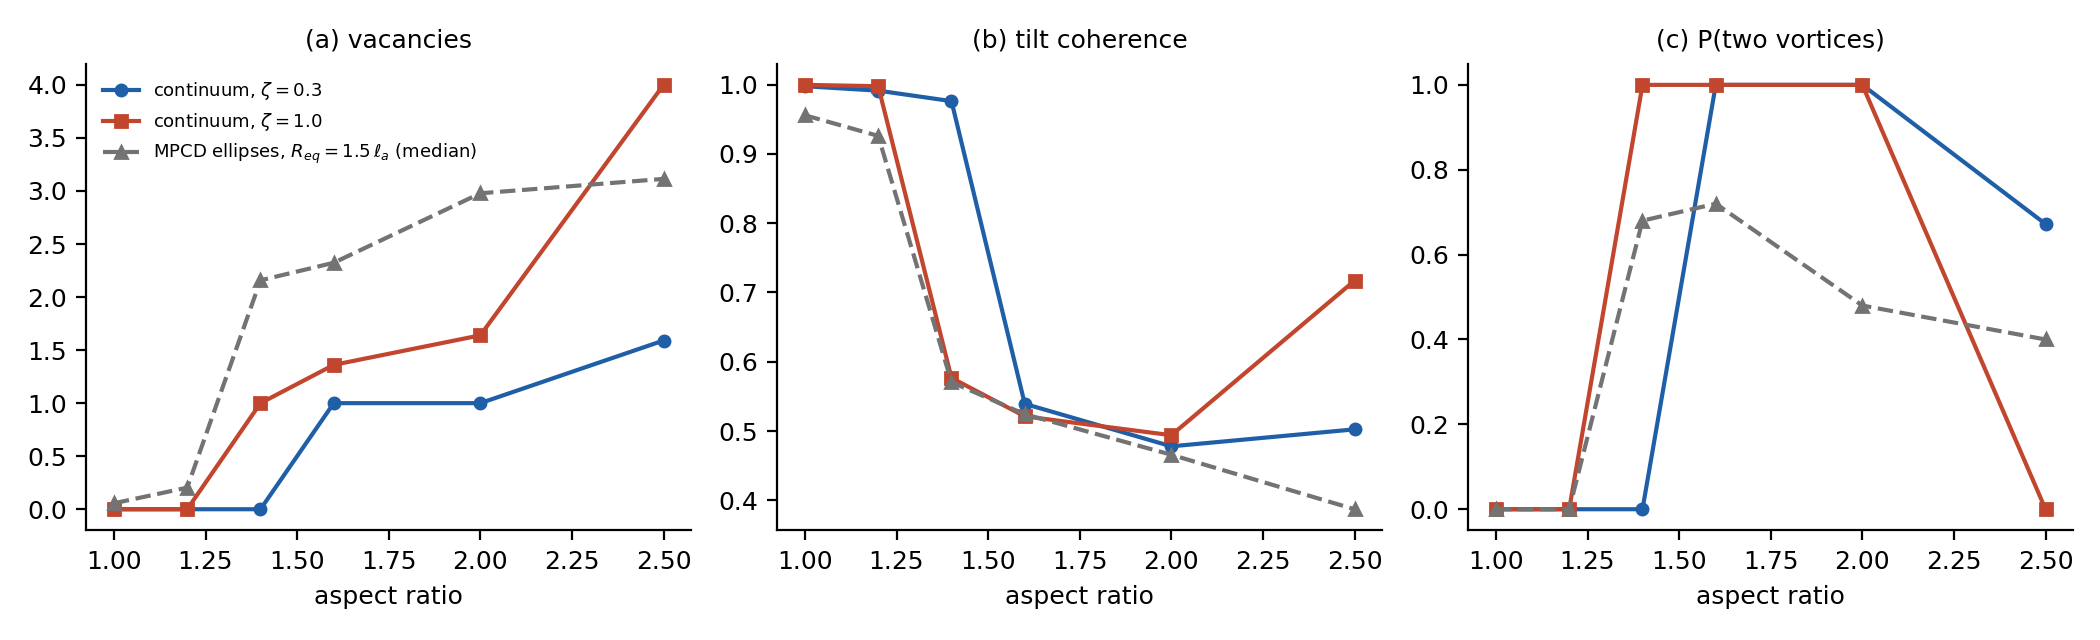
\includegraphics[width=\textwidth]{fig_cont_ellipse.png}
\caption{Active continuum model in ellipses (two activities) against the MPCD ellipse sweep at $R_\mathrm{eq}=1.5\,\la$: (a) vacancies, (b) tilt coherence, (c) fraction of time with two vortices.}\label{fig:contell}
\end{figure}
